\documentclass[12pt, a4paper]{scrreprt}
\usepackage[margin=2.5cm]{geometry}
\usepackage[hidelinks]{hyperref}
\usepackage{graphicx,xcolor,listings,tikz,enumitem}
\usetikzlibrary{positioning, arrows.meta, shapes, fit}

\definecolor{codegreen}{rgb}{0,0.6,0}
\definecolor{codegray}{rgb}{0.5,0.5,0.5}
\definecolor{codepurple}{rgb}{0.58,0,0.82}
\definecolor{backcolour}{rgb}{0.95,0.95,0.92}

\lstdefinestyle{mystyle}{
    backgroundcolor=\color{backcolour},
    commentstyle=\color{codegreen},
    keywordstyle=\color{blue},
    stringstyle=\color{codepurple},
    basicstyle=\ttfamily\footnotesize,
    numbers=left,
    numbersep=5pt,
    breaklines=true,
    tabsize=2
}
\lstset{style=mystyle}

\newcommand{\faculty}{Faculty Applied Information Technology}
\newcommand{\studies}{Bachelor of Cyber-Security}
\newcommand{\thesistitleDE}{Projekt "WeedDetector" \\ Arbeitsaufteilung \\ Christof Renner}
\newcommand{\submissiondate}{05.\ Juli 2025}
\newcommand{\supervisor}{Prof.\ Dr.\ Holger Jehle}

\begin{document}

\begin{titlepage}
  \centering
  {\LARGE Technische Hochschule Deggendorf \\ \faculty \par}
  \vspace{0.3cm}
  {\Large Studiengang \studies \\[1.5cm]}
  {\Huge\bfseries \thesistitleDE\par}
  \vfill
  \begin{minipage}[t]{0.45\textwidth}
    \textbf{Vorgelegt von:}\\
    \\
    Christof Renner (22301943)\\
    Manuel Friedl (1236626)\\
    \\
    \\
    \\
    \\
    Datum: \submissiondate
  \end{minipage}\hfill
  \begin{minipage}[t]{0.45\textwidth}
    \textbf{Prüfungsleitung:}\\
    \\
    \supervisor
  \end{minipage}
\end{titlepage}

\tableofcontents
\newpage

\chapter{Implementierung des Controllers}

Die WeedDetector-Anwendung basiert auf dem Model-View-Controller Modell. Die Entscheidung für MVC fiel aufgrund etablierter Industry Standards und erhöht somit Wartbarkeit, Erweiterbarkeit und Testbarkeit der Software.

\section{Zentrale Aufgaben des Controllers}

Im Rahmen der Anwendung erfüllt der Controller folgende wesentliche Funktionen:

\begin{itemize}
    \item \textbf{Ereignisgesteuerte Kommunikation:} Vermittelt zwischen GUI-Events und Modellaktionen, indem er Benutzereingaben weiterleitet und die Ergebnisse zurück zur GUI gibt.
    \item \textbf{Aktionsverarbeitung:} Reagiert auf spezifische Nutzeraktionen wie Bildauswahl, Start der Unkrauterkennung oder Steuerung des Roboters.
    \item \textbf{Robuste Fehlermechanismen:} Implementiert systematische Fehlerbehandlung zur Sicherstellung von Stabilität und Robustheit.
\end{itemize}

\section{Lose Kopplung durch Callback-Funktionen}

Um die Abhängigkeiten zwischen GUI und Controller minimal zu halten, nutzt der Controller sogenannte Callback-Funktionen, die bei bestimmten Ereignissen ausgelöst werden. Die Idee dahinter war die hohe Modularität des Vorgehens:

\begin{lstlisting}[language=Python, caption=Callback-Registrierung im Controller]
self.gui.on_select_image = self.handle_select_image
self.gui.on_detect = self.handle_detect
self.gui.on_start_robot = self.handle_start_robot
self.gui.on_stop_robot = self.handle_stop_robot
\end{lstlisting}

\begin{figure}[h!]
    \centering
    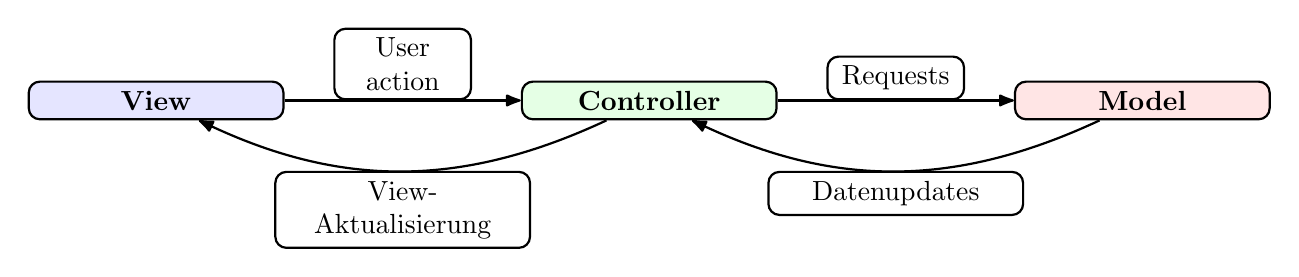
\begin{tikzpicture}[
        scale= 1.0,            % shrink everything to 70%
        transform shape,      % apply the scale to node shapes & text
        node distance=3 cm and 3cm,
        every node/.style={draw, text width=3cm, align=center, rounded corners},
        every path/.style={draw, thick, -{Latex[round]}}
    ]

    % Nodes
    \node (view) [fill=blue!10] {\textbf{View}\\};
    \node (controller) [right=of view, fill=green!10] {\textbf{Controller}\\};
    \node (model) [right=of controller, fill=red!10] {\textbf{Model}\\};

    % Arrows
  \path (view) -- node[above,text width=1.5cm]{User action} (controller);
  \path (controller) -- node[above,text width=1.5cm]{Requests} (model);
    \path (model) to[bend left=25] node[below]{Datenupdates} (controller);
    \path (controller) to[bend left=25] node[below]{View-Aktualisierung} (view);

    \end{tikzpicture}
    \caption{MVC-Architektur der WeedDetector-Anwendung}
    \label{fig:mvc-diagramm}
\end{figure}


\chapter{Modell, Dataset und Training}

\section{YOLO Modellarchitektur}
Das verwendete YOLO-Modell wurde aufgrund seiner ausgewogenen Balance zwischen Geschwindigkeit und Genauigkeit gewählt. Es eignet sich hervorragend zur Echtzeiterkennung verschiedener Unkrautarten.

\section{Datasetbeschreibung}
Die Trainingsdaten umfassen 13.349 Bilder, exportiert über Roboflow im YOLO-Format (640×640 Pixel). Die Augmentierung wurde über die Online-Plattform "Roboflow" durchgeführt und die Bilder anschließend lokal trainiert.

\section{Vorverarbeitungsschritte}
Folgende Vorverarbeitungsschritte wurden durchgeführt:
\begin{itemize}
    \item Auto-Orientierung zur Normalisierung der Bildausrichtung
    \item Größenanpassung auf 640×640 Pixel (Stretch)
    \item Automatische Kontrastanpassung mittels adaptiver Equalisierung
\end{itemize}

\section{Bildaugmentierung}
Zur Verbesserung der Generalisierung wurden umfangreiche Augmentierungen vorgenommen, sodass aus jedem Originalbild drei Trainingsvarianten entstanden:
\begin{itemize}
    \item Horizontale Spiegelung mit 50\% Wahrscheinlichkeit
    \item 90° Rotation (zufällig, Uhrzeiger- und Gegenuhrzeigersinn)
    \item Zufällige Rotation zwischen -15° und +15°
    \item Zufällige Ausschnitte (Crop) zwischen 0\% und 20\%
    \item Zufällige Anpassung von Sättigung (±20\%) und Belichtung (±10\%)
\end{itemize}

\chapter{Security und Linting}

\section{Statische Codeanalyse}
Wir setzen im Bereich Security auf statische Codeanalyse, dabei verwenden wir zur Analy- se zum einen "Bandit" und "snyk". Die Entscheidung wurde dabei auf Basis von bisherigen Erfahrungen und aufgrund der weiten Verbreitung der Tools, gerade im Pythonumfeld, getätigt.

\begin{lstlisting}[language=Bash, caption=Bandit via GitHub Actions]
- uses: actions/setup-python@v4
  with: {python-version: '3.x'}
- run: pip install bandit
- run: bandit -r . --skip trojansource
\end{lstlisting}
\noindent
Ergebnisse werden automatisiert bereitgestellt und im Falle von Auffälligkeiten als Issues behandelt.

\section{Python Linting}
Pylint analysiert kontinuierlich den Python-Code und prüft dabei auf Codequalität, Wartbarkeit, Fehleranfälligkeit und Einhaltung der PEP8-Konventionen. Auch wenn Linter nicht direkt securityrelevant sind, stellen wir so sicher, dass sauberer, strukturierter Code produziert wird.

\begin{lstlisting}[language=Bash, caption=Pylint Integration]
- uses: actions/setup-python@v5
  with: {python-version: '3.13'}
- run: pip install pylint
- run: pylint $(git ls-files '*.py')
\end{lstlisting}

\section{Dockerfile Linting}
Neben Python haben wir auch die Dockerfile mit Hadolint geprüft, um Best-Practices einzuhalten und potenzielle Schwachstellen auszuschließen:

\begin{lstlisting}[language=Bash, caption=Hadolint Action für Dockerfile]
- uses: hadolint/hadolint-action@v3.1.0
  with: {dockerfile: Dockerfile}
\end{lstlisting}

\newpage

\section{Dependency Management}
Für unser Dependency Management haben wir uns aus der nativen GitHub "All-in-One"-Lösung "dependabot" bedient, damit decken wir in alle dependencies über Docker, Python und GitHub Actions alles automatisiert ab.

\begin{lstlisting}[language=Bash, caption=Bandit via GitHub Actions]
version: 2
updates:
  - package-ecosystem: "pip"
    directory: "/"
    schedule:
      interval: "weekly"
    open-pull-requests-limit: 10
    labels:
      - "dependencies"
      - "python"
    
  - package-ecosystem: "docker"
    directory: "/"
    schedule:
      interval: "weekly"
    open-pull-requests-limit: 5
    labels:
      - "dependencies"
      - "docker"
      
  - package-ecosystem: "github-actions"
    directory: "/"
    schedule:
      interval: "weekly"
    open-pull-requests-limit: 5
    labels:
      - "dependencies"
      - "github-actions"
\end{lstlisting}

\section{Deployment}
Das Deployment des Dockerimages erfolgt über eine GitHub Action bei jedem Update der Dockerfile in die Docker registry. Dort wird in der Pipeline jeweils ein Lint-Prozess und ein Build-Prozess ausgeführt, somit wird verifiziert, dass sich der Container in einem optimalen Zustand für jeden Release befindet.

\begin{lstlisting}[language=Bash, caption=Bandit via GitHub Actions]
      - name: Build and push Docker image
        uses: docker/build-push-action@v6
        with:
          context: .
          push: true
          tags: crnnr/weeddetector:latest
\end{lstlisting}

\end{document}
